\documentclass[twoside]{book}

% Packages required by doxygen
\usepackage{calc}
\usepackage{doxygen}
\usepackage{graphicx}
\usepackage[utf8]{inputenc}
\usepackage{makeidx}
\usepackage{multicol}
\usepackage{multirow}
\usepackage{textcomp}
\usepackage[table]{xcolor}

% Font selection
\usepackage[T1]{fontenc}
\usepackage{mathptmx}
\usepackage[scaled=.90]{helvet}
\usepackage{courier}
\usepackage{amssymb}
\usepackage{sectsty}
\renewcommand{\familydefault}{\sfdefault}
\allsectionsfont{%
  \fontseries{bc}\selectfont%
  \color{darkgray}%
}
\renewcommand{\DoxyLabelFont}{%
  \fontseries{bc}\selectfont%
  \color{darkgray}%
}

% Page & text layout
\usepackage{geometry}
\geometry{%
  a4paper,%
  top=2.5cm,%
  bottom=2.5cm,%
  left=2.5cm,%
  right=2.5cm%
}
\tolerance=750
\hfuzz=15pt
\hbadness=750
\setlength{\emergencystretch}{15pt}
\setlength{\parindent}{0cm}
\setlength{\parskip}{0.2cm}
\makeatletter
\renewcommand{\paragraph}{%
  \@startsection{paragraph}{4}{0ex}{-1.0ex}{1.0ex}{%
    \normalfont\normalsize\bfseries\SS@parafont%
  }%
}
\renewcommand{\subparagraph}{%
  \@startsection{subparagraph}{5}{0ex}{-1.0ex}{1.0ex}{%
    \normalfont\normalsize\bfseries\SS@subparafont%
  }%
}
\makeatother

% Headers & footers
\usepackage{fancyhdr}
\pagestyle{fancyplain}
\fancyhead[LE]{\fancyplain{}{\bfseries\thepage}}
\fancyhead[CE]{\fancyplain{}{}}
\fancyhead[RE]{\fancyplain{}{\bfseries\leftmark}}
\fancyhead[LO]{\fancyplain{}{\bfseries\rightmark}}
\fancyhead[CO]{\fancyplain{}{}}
\fancyhead[RO]{\fancyplain{}{\bfseries\thepage}}
\fancyfoot[LE]{\fancyplain{}{}}
\fancyfoot[CE]{\fancyplain{}{}}
\fancyfoot[RE]{\fancyplain{}{\bfseries\scriptsize Generated on Tue Apr 15 2014 14\-:34\-:40 for Covert Collisions by Doxygen }}
\fancyfoot[LO]{\fancyplain{}{\bfseries\scriptsize Generated on Tue Apr 15 2014 14\-:34\-:40 for Covert Collisions by Doxygen }}
\fancyfoot[CO]{\fancyplain{}{}}
\fancyfoot[RO]{\fancyplain{}{}}
\renewcommand{\footrulewidth}{0.4pt}
\renewcommand{\chaptermark}[1]{%
  \markboth{#1}{}%
}
\renewcommand{\sectionmark}[1]{%
  \markright{\thesection\ #1}%
}

% Indices & bibliography
\usepackage{natbib}
\usepackage[titles]{tocloft}
\setcounter{tocdepth}{3}
\setcounter{secnumdepth}{5}
\makeindex

% Hyperlinks (required, but should be loaded last)
\usepackage{ifpdf}
\ifpdf
  \usepackage[pdftex,pagebackref=true]{hyperref}
\else
  \usepackage[ps2pdf,pagebackref=true]{hyperref}
\fi
\hypersetup{%
  colorlinks=true,%
  linkcolor=blue,%
  citecolor=blue,%
  unicode%
}

% Custom commands
\newcommand{\clearemptydoublepage}{%
  \newpage{\pagestyle{empty}\cleardoublepage}%
}


%===== C O N T E N T S =====

\begin{document}

% Titlepage & ToC
\hypersetup{pageanchor=false}
\pagenumbering{roman}
\begin{titlepage}
\vspace*{7cm}
\begin{center}%
{\Large Covert Collisions }\\
\vspace*{1cm}
{\large Generated by Doxygen 1.8.5}\\
\vspace*{0.5cm}
{\small Tue Apr 15 2014 14:34:40}\\
\end{center}
\end{titlepage}
\clearemptydoublepage
\tableofcontents
\clearemptydoublepage
\pagenumbering{arabic}
\hypersetup{pageanchor=true}

%--- Begin generated contents ---
\chapter{File Index}
\section{File List}
Here is a list of all files with brief descriptions\-:\begin{DoxyCompactList}
\item\contentsline{section}{/home/z\-Zelman/\-Dropbox/2\-D-\/\-Game\-Engine/src/\hyperlink{GameElement__gravity_8cpp}{Game\-Element\-\_\-gravity.\-cpp} }{\pageref{GameElement__gravity_8cpp}}{}
\item\contentsline{section}{/home/z\-Zelman/\-Dropbox/2\-D-\/\-Game\-Engine/src/\hyperlink{GameElement__gravity_8h}{Game\-Element\-\_\-gravity.\-h} }{\pageref{GameElement__gravity_8h}}{}
\item\contentsline{section}{/home/z\-Zelman/\-Dropbox/2\-D-\/\-Game\-Engine/src/\hyperlink{GameElement__movable_8cpp}{Game\-Element\-\_\-movable.\-cpp} }{\pageref{GameElement__movable_8cpp}}{}
\item\contentsline{section}{/home/z\-Zelman/\-Dropbox/2\-D-\/\-Game\-Engine/src/\hyperlink{GameElement__movable_8h}{Game\-Element\-\_\-movable.\-h} }{\pageref{GameElement__movable_8h}}{}
\item\contentsline{section}{/home/z\-Zelman/\-Dropbox/2\-D-\/\-Game\-Engine/src/\hyperlink{GameElement__static_8cpp}{Game\-Element\-\_\-static.\-cpp} }{\pageref{GameElement__static_8cpp}}{}
\item\contentsline{section}{/home/z\-Zelman/\-Dropbox/2\-D-\/\-Game\-Engine/src/\hyperlink{GameElement__static_8h}{Game\-Element\-\_\-static.\-h} }{\pageref{GameElement__static_8h}}{}
\item\contentsline{section}{/home/z\-Zelman/\-Dropbox/2\-D-\/\-Game\-Engine/src/\hyperlink{include__sfml_8h}{include\-\_\-sfml.\-h} }{\pageref{include__sfml_8h}}{}
\item\contentsline{section}{/home/z\-Zelman/\-Dropbox/2\-D-\/\-Game\-Engine/src/\hyperlink{main_8cpp}{main.\-cpp} }{\pageref{main_8cpp}}{}
\item\contentsline{section}{/home/z\-Zelman/\-Dropbox/2\-D-\/\-Game\-Engine/src/\-Graphic/\hyperlink{CAnimatable_8h}{C\-Animatable.\-h} }{\pageref{CAnimatable_8h}}{}
\item\contentsline{section}{/home/z\-Zelman/\-Dropbox/2\-D-\/\-Game\-Engine/src/\-Graphic/\hyperlink{CRenderable_8h}{C\-Renderable.\-h} }{\pageref{CRenderable_8h}}{}
\item\contentsline{section}{/home/z\-Zelman/\-Dropbox/2\-D-\/\-Game\-Engine/src/\-Graphic/\hyperlink{CSprite_8h}{C\-Sprite.\-h} }{\pageref{CSprite_8h}}{}
\item\contentsline{section}{/home/z\-Zelman/\-Dropbox/2\-D-\/\-Game\-Engine/src/\-Graphic/\hyperlink{CTexture_8h}{C\-Texture.\-h} }{\pageref{CTexture_8h}}{}
\item\contentsline{section}{/home/z\-Zelman/\-Dropbox/2\-D-\/\-Game\-Engine/src/\-Graphic/\hyperlink{RenderEngine_8h}{Render\-Engine.\-h} }{\pageref{RenderEngine_8h}}{}
\item\contentsline{section}{/home/z\-Zelman/\-Dropbox/2\-D-\/\-Game\-Engine/src/\-Graphic/\-Engine/\hyperlink{RenderEngine_8cpp}{Render\-Engine.\-cpp} }{\pageref{RenderEngine_8cpp}}{}
\item\contentsline{section}{/home/z\-Zelman/\-Dropbox/2\-D-\/\-Game\-Engine/src/\-Graphic/\-Objects/\hyperlink{CAnimatable_8cpp}{C\-Animatable.\-cpp} }{\pageref{CAnimatable_8cpp}}{}
\item\contentsline{section}{/home/z\-Zelman/\-Dropbox/2\-D-\/\-Game\-Engine/src/\-Graphic/\-Objects/\hyperlink{CRenderable_8cpp}{C\-Renderable.\-cpp} }{\pageref{CRenderable_8cpp}}{}
\item\contentsline{section}{/home/z\-Zelman/\-Dropbox/2\-D-\/\-Game\-Engine/src/\-Graphic/\-Objects/\hyperlink{CSprite_8cpp}{C\-Sprite.\-cpp} }{\pageref{CSprite_8cpp}}{}
\item\contentsline{section}{/home/z\-Zelman/\-Dropbox/2\-D-\/\-Game\-Engine/src/\-Graphic/\-Objects/\hyperlink{CTexture_8cpp}{C\-Texture.\-cpp} }{\pageref{CTexture_8cpp}}{}
\item\contentsline{section}{/home/z\-Zelman/\-Dropbox/2\-D-\/\-Game\-Engine/src/\-Physics/\hyperlink{CCollidable_8h}{C\-Collidable.\-h} }{\pageref{CCollidable_8h}}{}
\item\contentsline{section}{/home/z\-Zelman/\-Dropbox/2\-D-\/\-Game\-Engine/src/\-Physics/\hyperlink{CGravityBased_8h}{C\-Gravity\-Based.\-h} }{\pageref{CGravityBased_8h}}{}
\item\contentsline{section}{/home/z\-Zelman/\-Dropbox/2\-D-\/\-Game\-Engine/src/\-Physics/\hyperlink{CMovable_8h}{C\-Movable.\-h} }{\pageref{CMovable_8h}}{}
\item\contentsline{section}{/home/z\-Zelman/\-Dropbox/2\-D-\/\-Game\-Engine/src/\-Physics/\hyperlink{PhysicsEngine_8h}{Physics\-Engine.\-h} }{\pageref{PhysicsEngine_8h}}{}
\item\contentsline{section}{/home/z\-Zelman/\-Dropbox/2\-D-\/\-Game\-Engine/src/\-Physics/\-Engine/\hyperlink{PhysicsEngine_8cpp}{Physics\-Engine.\-cpp} }{\pageref{PhysicsEngine_8cpp}}{}
\item\contentsline{section}{/home/z\-Zelman/\-Dropbox/2\-D-\/\-Game\-Engine/src/\-Physics/\-Engine/\hyperlink{TRect_8h}{T\-Rect.\-h} }{\pageref{TRect_8h}}{}
\item\contentsline{section}{/home/z\-Zelman/\-Dropbox/2\-D-\/\-Game\-Engine/src/\-Physics/\-Objects/\hyperlink{CCollidable_8cpp}{C\-Collidable.\-cpp} }{\pageref{CCollidable_8cpp}}{}
\item\contentsline{section}{/home/z\-Zelman/\-Dropbox/2\-D-\/\-Game\-Engine/src/\-Physics/\-Objects/\hyperlink{CGravityBased_8cpp}{C\-Gravity\-Based.\-cpp} }{\pageref{CGravityBased_8cpp}}{}
\item\contentsline{section}{/home/z\-Zelman/\-Dropbox/2\-D-\/\-Game\-Engine/src/\-Physics/\-Objects/\hyperlink{CMovable_8cpp}{C\-Movable.\-cpp} }{\pageref{CMovable_8cpp}}{}
\end{DoxyCompactList}

\chapter{File Documentation}
\hypertarget{main_8cpp}{\section{/home/z\-Zelman/\-Dropbox/2\-D-\/\-Game\-Engine/src/main.cpp File Reference}
\label{main_8cpp}\index{/home/z\-Zelman/\-Dropbox/2\-D-\/\-Game\-Engine/src/main.\-cpp@{/home/z\-Zelman/\-Dropbox/2\-D-\/\-Game\-Engine/src/main.\-cpp}}
}
{\ttfamily \#include \char`\"{}include\-\_\-sfml.\-h\char`\"{}}\\*
{\ttfamily \#include \char`\"{}Graphic/\-C\-Texture.\-h\char`\"{}}\\*
{\ttfamily \#include \char`\"{}Graphic/\-C\-Sprite.\-h\char`\"{}}\\*
{\ttfamily \#include \char`\"{}Game\-Element\-\_\-movable.\-h\char`\"{}}\\*
{\ttfamily \#include \char`\"{}Game\-Element\-\_\-static.\-h\char`\"{}}\\*
{\ttfamily \#include \char`\"{}Physics/\-Physics\-Engine.\-h\char`\"{}}\\*
Include dependency graph for main.\-cpp\-:
\nopagebreak
\begin{figure}[H]
\begin{center}
\leavevmode
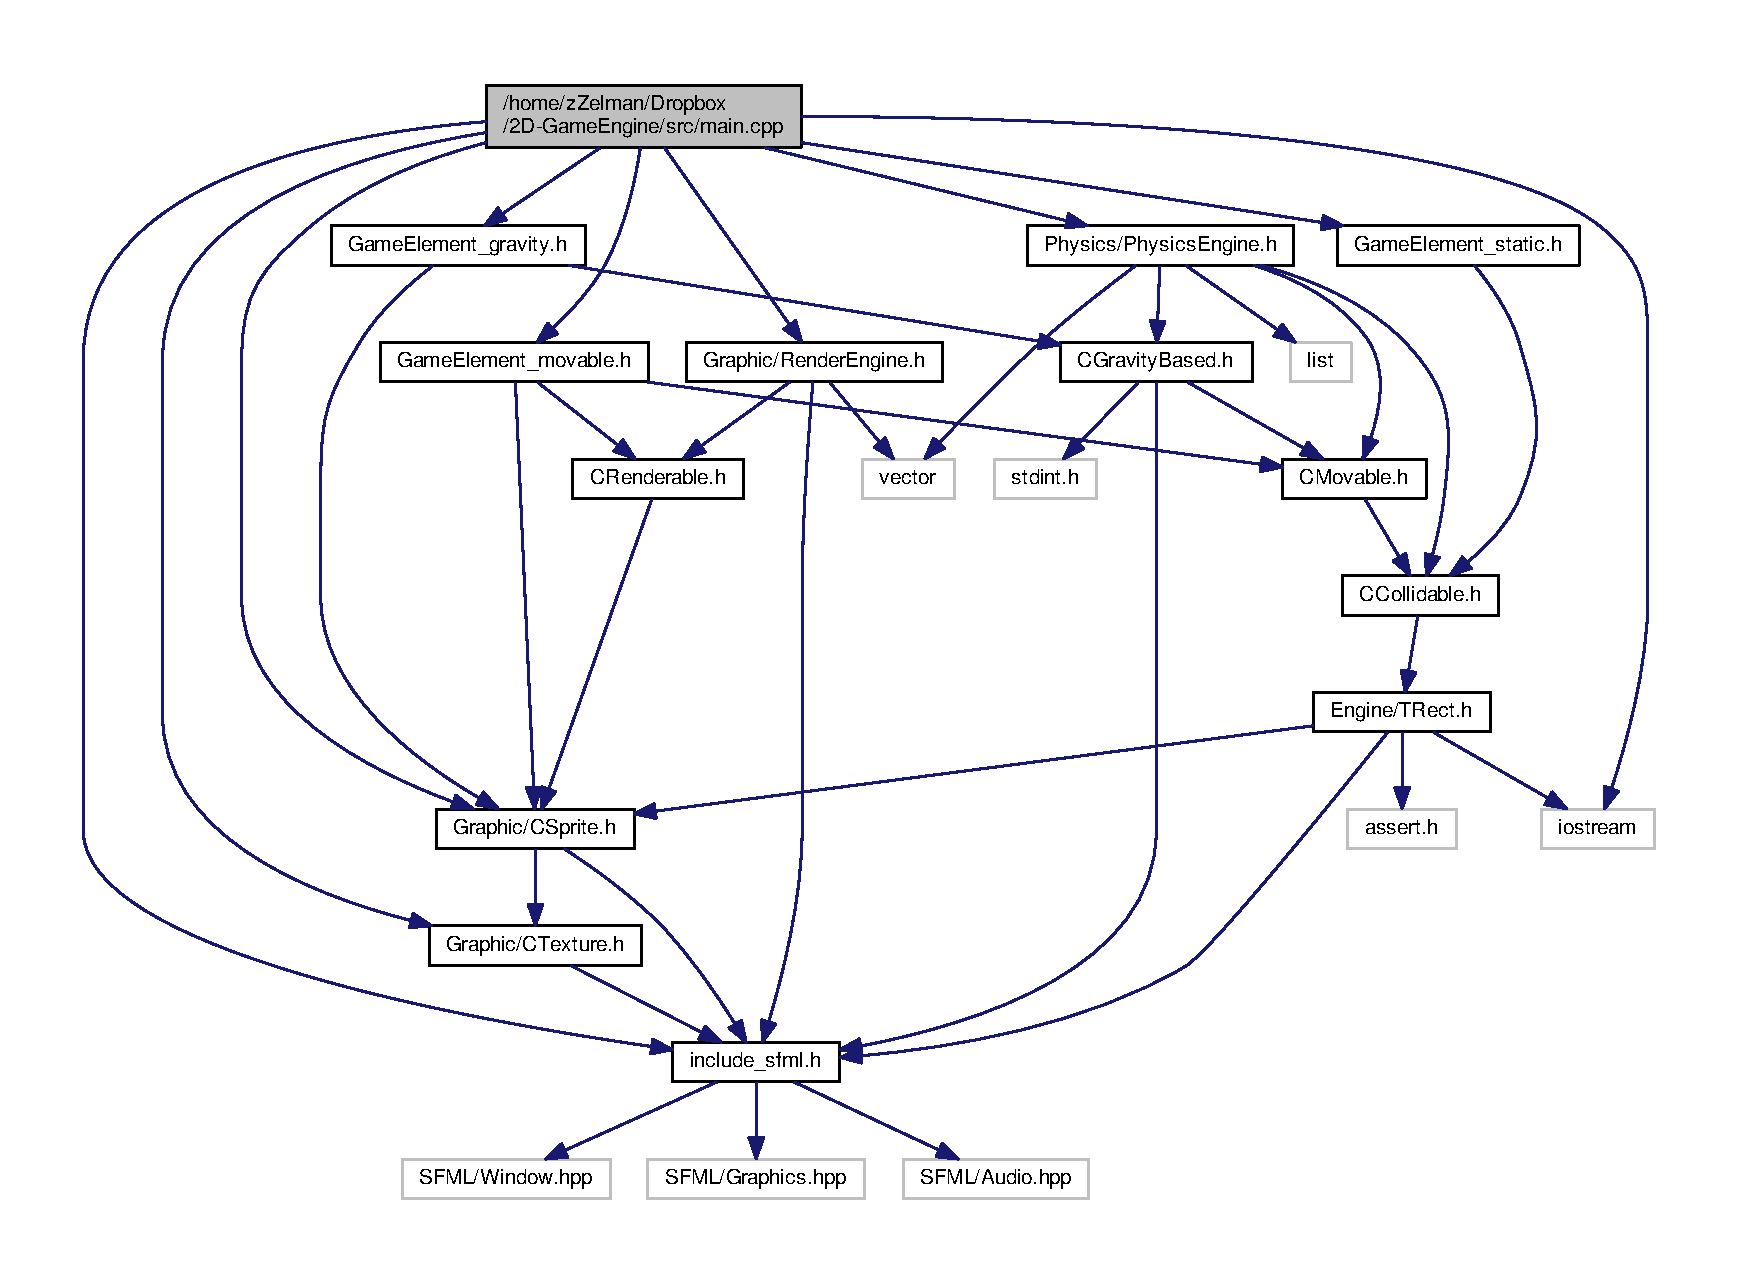
\includegraphics[width=350pt]{main_8cpp__incl}
\end{center}
\end{figure}
\subsection*{Functions}
\begin{DoxyCompactItemize}
\item 
void \hyperlink{main_8cpp_a0a462ec35bf9c8a31ea7b4c653ab3f4c}{window\-\_\-events} (bool \&done)
\begin{DoxyCompactList}\small\item\em Simplistic window event handling. \end{DoxyCompactList}\item 
void \hyperlink{main_8cpp_a6bbf2b1b4a5441f0205c3258bd661077}{update\-\_\-elements} ()
\begin{DoxyCompactList}\small\item\em Simplistic updating. \end{DoxyCompactList}\item 
void \hyperlink{main_8cpp_a20e3a3051df36234b0ce05ffac0741ee}{render\-\_\-elements} ()
\begin{DoxyCompactList}\small\item\em Simplistic rendering. \end{DoxyCompactList}\item 
void \hyperlink{main_8cpp_a190163a6c0c635f4695f2fdd61d2cb8c}{init\-\_\-elements} ()
\begin{DoxyCompactList}\small\item\em Init unit testing objects. \end{DoxyCompactList}\item 
void \hyperlink{main_8cpp_a4e306517e52618c9e9ba61f2beae2f94}{delete\-\_\-elements} ()
\begin{DoxyCompactList}\small\item\em Delete unit testing objects. \end{DoxyCompactList}\item 
int \hyperlink{main_8cpp_a0ddf1224851353fc92bfbff6f499fa97}{main} (int argc, char $\ast$argv\mbox{[}$\,$\mbox{]})
\begin{DoxyCompactList}\small\item\em Start of program. \end{DoxyCompactList}\end{DoxyCompactItemize}
\subsection*{Variables}
\begin{DoxyCompactItemize}
\item 
sf\-::\-Render\-Window $\ast$ \hyperlink{main_8cpp_a09bf53be0697112e73cc7ceaca479ef6}{g\-\_\-window}
\item 
\hyperlink{classCTexture}{C\-Texture} $\ast$ \hyperlink{main_8cpp_a7e2879f22f371962a365e7c8d9f0699f}{g\-\_\-texture}
\item 
\hyperlink{classCSprite}{C\-Sprite} $\ast$ \hyperlink{main_8cpp_a68ec2c6cb385b95c73463cbeeb11759d}{g\-\_\-sprite\-\_\-movable}
\item 
\hyperlink{classGameElement__movable}{Game\-Element\-\_\-movable} $\ast$ \hyperlink{main_8cpp_ab43805fb979ee1bdb9fa4ef8500736f5}{g\-\_\-element\-\_\-movable}
\item 
\hyperlink{classCSprite}{C\-Sprite} $\ast$ \hyperlink{main_8cpp_acb23cd68aed5278e47711f5b62734397}{g\-\_\-sprite\-\_\-static}
\item 
\hyperlink{classGameElement__static}{Game\-Element\-\_\-static} $\ast$ \hyperlink{main_8cpp_aff6119240a4bf77d3a20abd24127b596}{g\-\_\-element\-\_\-static}
\item 
\hyperlink{classengine_1_1PhysicsEngine}{engine\-::\-Physics\-Engine} $\ast$ \hyperlink{main_8cpp_aee1bcd5912424a8845145c705c1e3e39}{g\-\_\-physics\-Engine}
\end{DoxyCompactItemize}


\subsection{Function Documentation}
\hypertarget{main_8cpp_a4e306517e52618c9e9ba61f2beae2f94}{\index{main.\-cpp@{main.\-cpp}!delete\-\_\-elements@{delete\-\_\-elements}}
\index{delete\-\_\-elements@{delete\-\_\-elements}!main.cpp@{main.\-cpp}}
\subsubsection[{delete\-\_\-elements}]{\setlength{\rightskip}{0pt plus 5cm}void delete\-\_\-elements (
\begin{DoxyParamCaption}
{}
\end{DoxyParamCaption}
)}}\label{main_8cpp_a4e306517e52618c9e9ba61f2beae2f94}


Delete unit testing objects. 



Definition at line 135 of file main.\-cpp.

\hypertarget{main_8cpp_a190163a6c0c635f4695f2fdd61d2cb8c}{\index{main.\-cpp@{main.\-cpp}!init\-\_\-elements@{init\-\_\-elements}}
\index{init\-\_\-elements@{init\-\_\-elements}!main.cpp@{main.\-cpp}}
\subsubsection[{init\-\_\-elements}]{\setlength{\rightskip}{0pt plus 5cm}void init\-\_\-elements (
\begin{DoxyParamCaption}
{}
\end{DoxyParamCaption}
)}}\label{main_8cpp_a190163a6c0c635f4695f2fdd61d2cb8c}


Init unit testing objects. 



Definition at line 110 of file main.\-cpp.

\hypertarget{main_8cpp_a0ddf1224851353fc92bfbff6f499fa97}{\index{main.\-cpp@{main.\-cpp}!main@{main}}
\index{main@{main}!main.cpp@{main.\-cpp}}
\subsubsection[{main}]{\setlength{\rightskip}{0pt plus 5cm}int main (
\begin{DoxyParamCaption}
\item[{int}]{argc, }
\item[{char $\ast$}]{argv\mbox{[}$\,$\mbox{]}}
\end{DoxyParamCaption}
)}}\label{main_8cpp_a0ddf1224851353fc92bfbff6f499fa97}


Start of program. 



Definition at line 154 of file main.\-cpp.

\hypertarget{main_8cpp_a20e3a3051df36234b0ce05ffac0741ee}{\index{main.\-cpp@{main.\-cpp}!render\-\_\-elements@{render\-\_\-elements}}
\index{render\-\_\-elements@{render\-\_\-elements}!main.cpp@{main.\-cpp}}
\subsubsection[{render\-\_\-elements}]{\setlength{\rightskip}{0pt plus 5cm}void render\-\_\-elements (
\begin{DoxyParamCaption}
{}
\end{DoxyParamCaption}
)}}\label{main_8cpp_a20e3a3051df36234b0ce05ffac0741ee}


Simplistic rendering. 



Definition at line 97 of file main.\-cpp.

\hypertarget{main_8cpp_a6bbf2b1b4a5441f0205c3258bd661077}{\index{main.\-cpp@{main.\-cpp}!update\-\_\-elements@{update\-\_\-elements}}
\index{update\-\_\-elements@{update\-\_\-elements}!main.cpp@{main.\-cpp}}
\subsubsection[{update\-\_\-elements}]{\setlength{\rightskip}{0pt plus 5cm}void update\-\_\-elements (
\begin{DoxyParamCaption}
{}
\end{DoxyParamCaption}
)}}\label{main_8cpp_a6bbf2b1b4a5441f0205c3258bd661077}


Simplistic updating. 



Definition at line 88 of file main.\-cpp.

\hypertarget{main_8cpp_a0a462ec35bf9c8a31ea7b4c653ab3f4c}{\index{main.\-cpp@{main.\-cpp}!window\-\_\-events@{window\-\_\-events}}
\index{window\-\_\-events@{window\-\_\-events}!main.cpp@{main.\-cpp}}
\subsubsection[{window\-\_\-events}]{\setlength{\rightskip}{0pt plus 5cm}void window\-\_\-events (
\begin{DoxyParamCaption}
\item[{bool \&}]{done}
\end{DoxyParamCaption}
)}}\label{main_8cpp_a0a462ec35bf9c8a31ea7b4c653ab3f4c}


Simplistic window event handling. 



Definition at line 22 of file main.\-cpp.



\subsection{Variable Documentation}
\hypertarget{main_8cpp_ab43805fb979ee1bdb9fa4ef8500736f5}{\index{main.\-cpp@{main.\-cpp}!g\-\_\-element\-\_\-movable@{g\-\_\-element\-\_\-movable}}
\index{g\-\_\-element\-\_\-movable@{g\-\_\-element\-\_\-movable}!main.cpp@{main.\-cpp}}
\subsubsection[{g\-\_\-element\-\_\-movable}]{\setlength{\rightskip}{0pt plus 5cm}{\bf Game\-Element\-\_\-movable}$\ast$ g\-\_\-element\-\_\-movable}}\label{main_8cpp_ab43805fb979ee1bdb9fa4ef8500736f5}


Definition at line 12 of file main.\-cpp.

\hypertarget{main_8cpp_aff6119240a4bf77d3a20abd24127b596}{\index{main.\-cpp@{main.\-cpp}!g\-\_\-element\-\_\-static@{g\-\_\-element\-\_\-static}}
\index{g\-\_\-element\-\_\-static@{g\-\_\-element\-\_\-static}!main.cpp@{main.\-cpp}}
\subsubsection[{g\-\_\-element\-\_\-static}]{\setlength{\rightskip}{0pt plus 5cm}{\bf Game\-Element\-\_\-static}$\ast$ g\-\_\-element\-\_\-static}}\label{main_8cpp_aff6119240a4bf77d3a20abd24127b596}


Definition at line 15 of file main.\-cpp.

\hypertarget{main_8cpp_aee1bcd5912424a8845145c705c1e3e39}{\index{main.\-cpp@{main.\-cpp}!g\-\_\-physics\-Engine@{g\-\_\-physics\-Engine}}
\index{g\-\_\-physics\-Engine@{g\-\_\-physics\-Engine}!main.cpp@{main.\-cpp}}
\subsubsection[{g\-\_\-physics\-Engine}]{\setlength{\rightskip}{0pt plus 5cm}{\bf engine\-::\-Physics\-Engine}$\ast$ g\-\_\-physics\-Engine}}\label{main_8cpp_aee1bcd5912424a8845145c705c1e3e39}


Definition at line 17 of file main.\-cpp.

\hypertarget{main_8cpp_a68ec2c6cb385b95c73463cbeeb11759d}{\index{main.\-cpp@{main.\-cpp}!g\-\_\-sprite\-\_\-movable@{g\-\_\-sprite\-\_\-movable}}
\index{g\-\_\-sprite\-\_\-movable@{g\-\_\-sprite\-\_\-movable}!main.cpp@{main.\-cpp}}
\subsubsection[{g\-\_\-sprite\-\_\-movable}]{\setlength{\rightskip}{0pt plus 5cm}{\bf C\-Sprite}$\ast$ g\-\_\-sprite\-\_\-movable}}\label{main_8cpp_a68ec2c6cb385b95c73463cbeeb11759d}


Definition at line 11 of file main.\-cpp.

\hypertarget{main_8cpp_acb23cd68aed5278e47711f5b62734397}{\index{main.\-cpp@{main.\-cpp}!g\-\_\-sprite\-\_\-static@{g\-\_\-sprite\-\_\-static}}
\index{g\-\_\-sprite\-\_\-static@{g\-\_\-sprite\-\_\-static}!main.cpp@{main.\-cpp}}
\subsubsection[{g\-\_\-sprite\-\_\-static}]{\setlength{\rightskip}{0pt plus 5cm}{\bf C\-Sprite}$\ast$ g\-\_\-sprite\-\_\-static}}\label{main_8cpp_acb23cd68aed5278e47711f5b62734397}


Definition at line 14 of file main.\-cpp.

\hypertarget{main_8cpp_a7e2879f22f371962a365e7c8d9f0699f}{\index{main.\-cpp@{main.\-cpp}!g\-\_\-texture@{g\-\_\-texture}}
\index{g\-\_\-texture@{g\-\_\-texture}!main.cpp@{main.\-cpp}}
\subsubsection[{g\-\_\-texture}]{\setlength{\rightskip}{0pt plus 5cm}{\bf C\-Texture}$\ast$ g\-\_\-texture}}\label{main_8cpp_a7e2879f22f371962a365e7c8d9f0699f}


Definition at line 9 of file main.\-cpp.

\hypertarget{main_8cpp_a09bf53be0697112e73cc7ceaca479ef6}{\index{main.\-cpp@{main.\-cpp}!g\-\_\-window@{g\-\_\-window}}
\index{g\-\_\-window@{g\-\_\-window}!main.cpp@{main.\-cpp}}
\subsubsection[{g\-\_\-window}]{\setlength{\rightskip}{0pt plus 5cm}sf\-::\-Render\-Window$\ast$ g\-\_\-window}}\label{main_8cpp_a09bf53be0697112e73cc7ceaca479ef6}


Definition at line 8 of file main.\-cpp.


%--- End generated contents ---

% Index
\newpage
\phantomsection
\addcontentsline{toc}{part}{Index}
\printindex

\end{document}
